\chapter{System Design}
\section{Goals of Design}
\begin{enumerate}
 \item The project design should help us to visualize the system as it is or want it to be.
 \item It should permit us to specify the structure or behavior of the system.
 \item To give us template that guides us in the construction of the system.
 \item To document the decision we have made.
\end{enumerate}

\section{UML Diagrams}
\hspace*{0.82cm}The OMG's Unified Modeling Language (UML) helps specify, visualize, and
document models of software systems, including their structure and design, in a way that
meets all of these requirements. Using any one of the large number of UML-based tools on
the market, one can analyze future application's requirements and design a solution that meets
them, representing the results using UML's twelve standard diagram types. One can model
just about any type of application, running on any type and combination of hardware,
operating system, programming language, and network, in UML. Its flexibility helps model
distributed applications that use just about any middleware on the market. Built upon the
MOF metamodel which defines class and operation as fundamental concepts, it's a natural fit
for object-oriented languages and environments such as C++, Java and the recent C\#, but one
can use it to model non-OO applications as well in, for example, Fortran, VB, or COBOL.\\[0.5cm]
\hspace*{0.82cm}Architects design buildings. Builders use the designs to create buildings. The more
complicated the building, the more critical the communication between architect and builder.
Blueprints are the standard graphical language that both architects and builders must learn as
part of their trade.\\[0.5cm]
\hspace*{0.82cm}Writing software is not unlike constructing a building. The more complicated the
underlying system, the more critical the communication among everyone involved in creating
and deploying the software. In the past decade, the UML has emerged as the software
blueprint language for analysts, designers, and programmers alike. It is now part of the
software trade. The UML gives everyone from business analyst to designer to programmer a
common vocabulary to talk about software design.\\[0.5cm]
\hspace*{0.82cm}The UML is applicable to object-oriented problem solving. Anyone interested in
learning UML must be familiar with the underlying tenet of object-oriented problem solving 
it all begins with the construction of a model. A model is an abstraction of the underlying
problem. The domain is the actual world from which the problem comes.\\[0.5cm]
\hspace*{0.82cm}Models consist of objects that interact by sending each other message. Think of an
object as "alive." Objects have things they know (attributes) and things they can do
(behaviors or operations). The values of an object's attributes determine its state.\\[0.5cm]
\hspace*{0.82cm}Classes are the "blueprints" for objects. A class wraps attributes (data) and behaviors
(methods or functions) into a single distinct entity. Objects are instances of classes.\\[0.5cm]
At the center of the UML are its nine kinds of modeling diagrams, which we describe here.
\begin{itemize}
 \item Use case diagrams
 \item Class diagrams
 \item Object diagrams
 \item Sequence diagrams
 \item Collaboration diagrams
 \item Statechart diagrams
 \item Activity diagrams
 \item Component diagrams
 \item Deployment diagrams
\end{itemize}
To model our system we have used the following diagrams:\\[0.5cm]
\textbf{Class Diagram}\\
\hspace*{0.82cm}A Class diagram is type of structure diagram that describes
structure of our system by showing system classes, their attributes and relationships between
them. Class diagrams are important for visualizing, specifying and documenting structural
models.\\[1cm]
\begin{figure}[H]
  \centering
    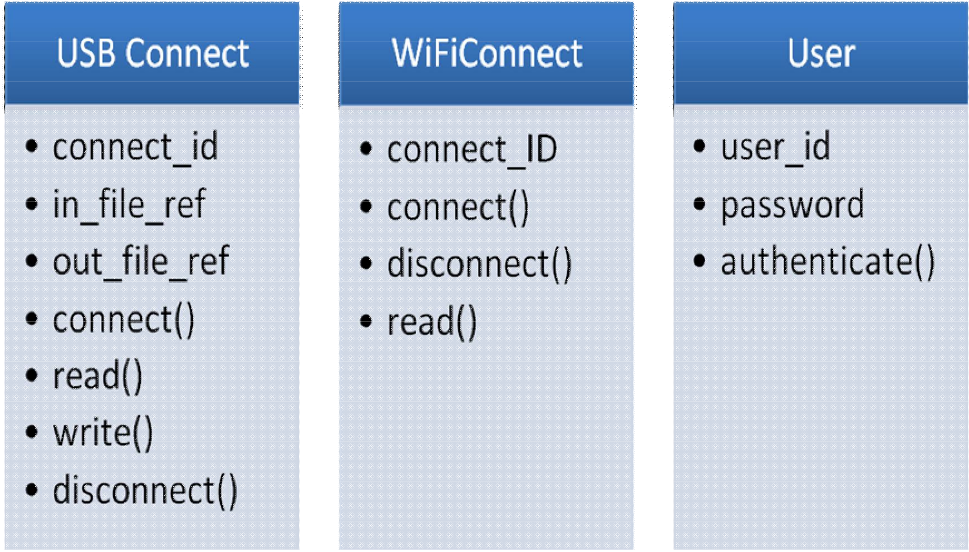
\includegraphics[height=7cm, width=12cm]{project/images/class-diagram}
  \caption{\textbf{Class Diagram}}
\end{figure}
\newpage
\textbf{Use Case Diagram}\\
\hspace*{0.82cm}Use case diagram are central to modeling the behavior of a system or class each one
shows a set of use cases and actors and their relationships. These model the users expectation
for using the system.\\[1cm]
\begin{figure}[H]
  \centering
    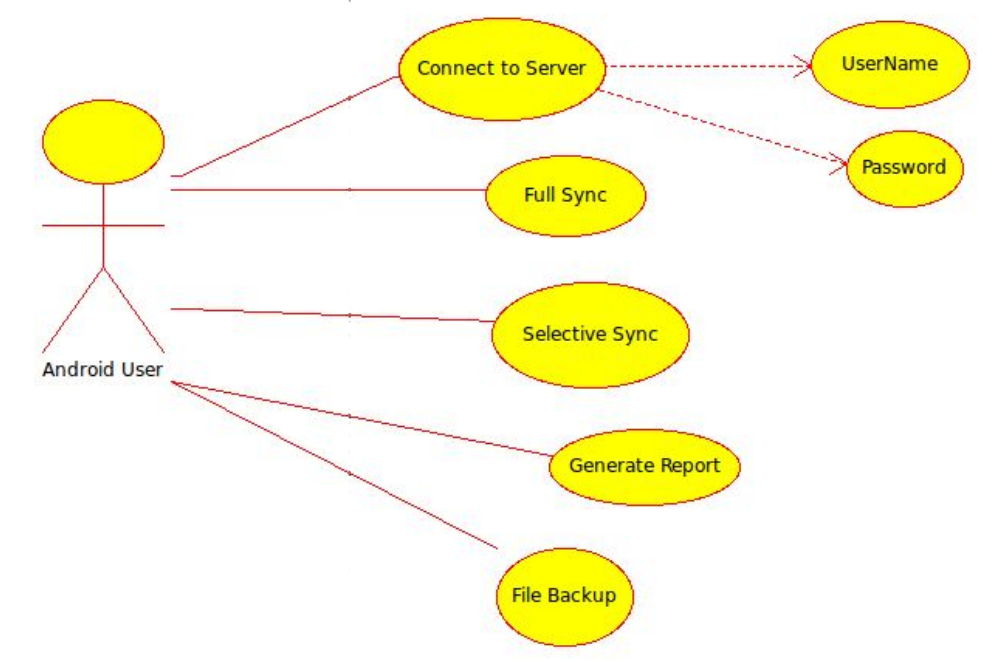
\includegraphics[height= 15cm, width=15cm]{project/images/use-case}
  \caption{\textbf{Use Case Diagram}}
\end{figure}
\newpage
\textbf{Sequence Diagram}\\
\hspace*{0.82cm}A sequence diagram in a Unified Modeling Language (UML) is a kind of interaction
diagram that shows how processes operate with one another and in what order. It is a
construct of a Message Sequence Chart. A sequence diagram shows object interactions
arranged in time sequence. It depicts the objects and classes involved in the scenario and the
sequence of messages exchanged between the objects needed to carry out the functionality of
the scenario. Sequence diagrams typically are associated with use case realizations in the
Logical View of the system under development.\\[1cm]
\begin{figure}[H]
  \centering
    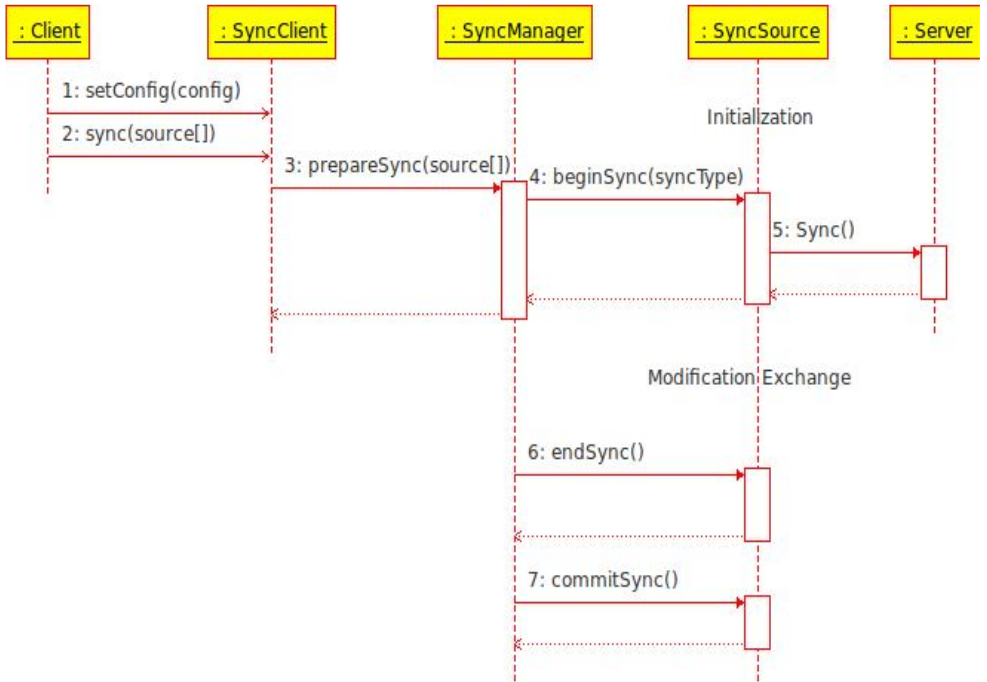
\includegraphics[height= 15cm, width=17cm]{project/images/seq-diagram}
  \caption{\textbf{Sequence Diagram}}
\end{figure}
\newpage
\section{Feasibility Study}
\hspace*{0.82cm}As we are developing our system we would like to consider the feasibility aspects of
this system. We are trying to develop a system which is an improvised version of the current
implementation. So while carrying out a feasibility study, we would like to compare our
proposed system with the current scenario.
\subsection{Current Implementation}
The current scenario is as follows:
\begin{enumerate}
 \item User logs onto his Google account.
 \item Synchronization starts and data are sent to the cloud.
 \item This data remains on third-party servers (Google)
 \item This data can be later retrieved from the cloud.
 \item This data can be later retrieved from the cloud.
\end{enumerate}
\subsection{The Proposed System}
\hspace*{0.82cm}As opposed to the current implementation, we want to increase the privacy of the
users by enabling them to save their data to be synchronized on their own private servers.
These private servers can be Desktop PCs, Laptops, etc.\\[0.5cm]
The steps would include:
\begin{enumerate}
 \item Ensure server is on
 \item Log onto the application on the server (for online mode)
 \item For offline mode, connect the device using USB cable, Wi-Fi, Bluetooth
 \item Start synchronization (full or selective sync)
 \item Log off
 \item This system is being developed keeping in mind the basic synchronization
necessities of the average android user. Hence it can be used by both average
users as well as large corporations to keep their employee data (on their android
mobile devices) safe.
% \item Thus it can be said that this system has large practical applications and has immense future scope.
\end{enumerate}